
%%%%%%%%%%%%%%%%%%%%%%%%%%%%%%%%%%%%%%%%%%%%%%%%%%%%%%%%%%%%%
%%%%%%%%%%%%%%%%%%%%%%%%%%%%%%%%%%%%%%%%%%%%%%%%%%%%%%%%%%%%%
%
%  %%%%%%%  %    %  %%%%%%  %%%%%%  %%%%%%%  %%%%%%%  %%%%%
%  %        %    %  %    %  %     %    %     %        %    %
%  %        %    %  %%%%%%  %     %    %     %        %    %
%  %        %%%%%%  %    %  %%%%%%     %     %%%%%    %%%%%
%  %        %    %  %    %  %          %     %        %    %
%  %%%%%%%  %    %  %    %  %          %     %%%%%%%  %     %
%
%%%%%%%%%%%%%%%%%%%%%%%%%%%%%%%%%%%%%%%%%%%%%%%%%%%%%%%%%%%%%
%%%%%%%%%%%%%%%%%%%%%%%%%%%%%%%%%%%%%%%%%%%%%%%%%%%%%%%%%%%%%

\chapter{A Metric on the Category of Sheaves}
\label{sec:metric}

\begin{quote}
$A\Gamma E\Omega METPHTO\Sigma \,\, MH\Delta EI\Sigma \,\,EI\Sigma I T\Omega$\footnote{``Let no one who cannot think geometrically enter.''~\cite{plato-academy}}
\begin{flushright} --- Purported Inscription at The Academy \end{flushright}
\end{quote}

Science depends on knowing that measurements and observations should only be trusted up to an interval of uncertainty. Saying that one is traveling about 30 miles per hour depends on their being a continuum of speeds. It makes no sense to say that one is traveling at a speed that happens to be an algebraic number.~\footnote{This metaphor was used by Bob MacPherson in his opening remarks on ``Continuity and the philosophy of science.''~\cite{macpherson-seminar}} Persistent homology has addressed this issue in a rather elegant way. Given two functions $f,g:Y\to\RR$ such that
\[
||f-g||_{\infty}:=\sup_{y}|f(y)-g(y)| < \epsilon
\]
one can say that the sublevel sets obey the inclusions
\[
f^{-1}(-\infty,t] \subset g^{-1}(-\infty,t+\epsilon] \qquad \mathrm{and} \qquad g^{-1}(-\infty,t] \subset t^{-1}(-\infty,t+\epsilon]
\]
for every value of $t$. In the language of~\cite{chazal2009proximity}, one has an \textbf{interleaving} of sublevel sets:
\[
\xymatrix{ f^{-1}(-\infty,t] \ar[dr] \ar[r] & f^{-1}(-\infty,t+\epsilon] \ar[dr] \ar[r] & f^{-1}(-\infty,t+2\epsilon] \\
g^{-1}(-\infty,t] \ar[ur] \ar[r] & g^{-1}(-\infty,t+\epsilon] \ar[ur] \ar[r] & g^{-1}(-\infty,t+2\epsilon]}
\]
By functoriality of homology, one obtains a notion of interleaving of functors in $\Fun(\RR,\Vect)$, where $\RR$ with its partial order is viewed as a category. Defining the interleaving distance to be the infimum over all $\epsilon$ such that there is an $\epsilon$-interleaving gives an extended pseudo-metric on the category of such functors.

In this chapter, we will consider a generalization of this approach, first for pre-sheaves and then for sheaves. We will try to answer analogous questions such as, ``Suppose we have two maps $f,g:Y\to X$ to a metric space that are close in the supremum norm, i.e.
\[
d_{\infty}(f,g)=\sup_{y\in Y} d_X(f(y),g(y)) < \epsilon.
\]
Is there any reasonable sense where the pushforward sheaves $f_*k_Y$ and $g_*k_Y$ are close?'' It turns out that the answer is ``yes,'' but studying higher invariants of the fiber, such as $H^i$ for $i\geq 1$, is unstable to large perturbations. By studying interleavings of complexes of sheaves, one obtains a derived stability result. To conclude the chapter, we provide preliminary results towards equating the interleaving distance with a modified version of the bottleneck distance described in~\cite{cohen2007stability} for definable sheaves with finite support over the real line. The most important takeaway from this chapter is that interleavings for sheaves and pre-sheaves are obstructed by global sections.

\begin{figure}
\centering
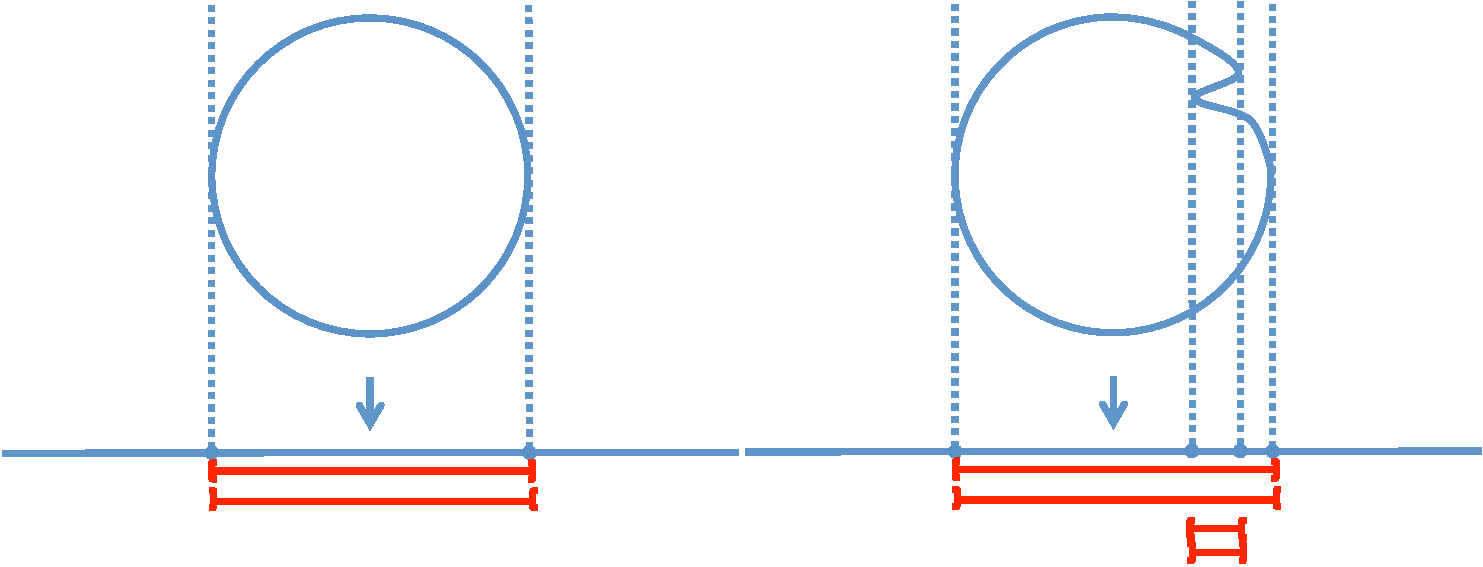
\includegraphics[width=\textwidth]{perturb.pdf}
\caption{Do Close Maps Give Rise to ``Close'' Sheaves?}
\label{fig:perturb}
\end{figure}

\section{Interleavings for Pre-Sheaves}

\begin{defn}\index{epsilon@$\epsilon$ thickening}
	Let $(X,d)$ be a metric space. The \textbf{$\epsilon$-thickening of open sets} is the map of posets
	\[
		\epsilon: \Open(X) \to \Open(X)
	\]
	given by
	\[
			U \rightsquigarrow U^{\epsilon}:=\cup_{x\in U} B(x,\epsilon).
	\]
	Of course, any map of posets dualizes to a map of posets $\epsilon:
	\Open(X)^{op}\to\Open(X)^{op}$
\end{defn}
\begin{rmk}
	For metric spaces like $\RR^n$ with the Euclidean metric, $(U^{\epsilon})^{\epsilon}=U^{2\epsilon}$. In general, the triangle inequality implies that $(U^{\epsilon})^{\epsilon}\subseteq U^{2\epsilon}$. The reverse containment is also true if $(X,d)$ is convex, for example. Convexity guarantees that intuitive results are true, but it is not strictly necessary for any of the following arguments.
\end{rmk}

\begin{defn}[Thickened Pre-Sheaf]
	Using the previous two definitions, we can define the \textbf{$\epsilon$-thickening of a pre-sheaf} $F$ via the formula
	\[
		F^{\epsilon}:=F\circ \epsilon \qquad \mathrm{i.e.} \qquad  F^{\epsilon}(U):=F(U^{\epsilon}).
	\]
	Moreover, the thickening operation is functorial. If $\varphi: F\to G$ is a natural transformation, then we get for free a natural transformation between the thickened pre-sheaves $\varphi_{\epsilon}:F^{\epsilon}\to G^{\epsilon}$. Consequently, we can define the \textbf{$\epsilon$-thickening functor} to be
	\[
		\epsilon^*:\Preshv(X)\to\Preshv(X) \qquad F \rightsquigarrow F^{\epsilon}.
	\]
\end{defn}
One of the most important observations for working with interleavings is that since $F$ is a pre-sheaf we have a canonical natural transformation
\[
	\eta^F_{\epsilon}:F^{\epsilon}\to F
\]
coming from $\rho_{U,U^{\epsilon}}:F^{\epsilon}(U)=F(U^{\epsilon})\to F(U)$. This follows by showing that for every pair $V\subseteq U$ the square
\[
	\xymatrix{ F^{\epsilon}(U) \ar[r]^{\rho_{U,U^{\epsilon}}} \ar[d]_{\rho_{V^{\epsilon},U^{\epsilon}}} & F(U) \ar[d]^{\rho_{V,U}} \\
	F^{\epsilon}(V) \ar[r]_{\rho_{V,V^{\epsilon}}} & F(V) }
\]
commutes by virtue of $F$ being a pre-sheaf:
\[
	\rho_{V,U}\circ \rho_{U,U^{\epsilon}}=\rho_{V,U^{\epsilon}}=\rho_{V,V^{\epsilon}}\circ \rho_{V^{\epsilon},U^{\epsilon}}
\]
Of course, the map
\[
	\eta^F_{2\epsilon}:F^{2\epsilon}\to F
\]
always exists as well and for metric spaces where $U^{2\epsilon}=(U^{\epsilon})^{\epsilon}$ it is equal to the composition $\eta^F_{\epsilon}\circ \epsilon^*\eta^F_{\epsilon}$.

\begin{rmk}[Notation $2\epsilon$ vs. $\epsilon\epsilon$]
To avoid cumbersome notation, we may sometimes substitute $U^{2\epsilon}$ for $(U^{\epsilon})^{\epsilon}$, $\eta^F_{2\epsilon}$ for $\epsilon^*\eta^F_{\epsilon}$, $F^{2\epsilon}$ for $\epsilon^*F^{\epsilon}$, and so on. For metric spaces such as $\RR^n$ with the Euclidean metric these differences do not exist and can be safely ignored.
\end{rmk}

A version of the following definition was communicated to the author by Amit Patel~\cite{patel}.

\begin{defn}[Interleaving of Pre-Sheaves]\index{interleaving!of presheaves}
	Let $F,G:\Open(X)^{op}\to\dat$ be two pre-sheaves on a metric space $X$. We define an \textbf{$\epsilon$-interleaving} of $F$ and $G$ to be a pair of natural transformations 
	\[
	\varphi_{\epsilon}:F^{\epsilon}\to G \qquad \psi_{\epsilon}: G^{\epsilon}\to F
	\]
	that satisfy the compatibility relations
	\[
		\eta^F_{2\epsilon}=\psi_{\epsilon}\circ \epsilon^*\varphi_{\epsilon} \qquad \eta^G_{2\epsilon}=\varphi_{\epsilon}\circ \epsilon^*\psi_{\epsilon}.
	\]
	An interleaving is better summarized via the following commutative diagram:
	\[
	\xymatrix{F^{2\epsilon} \ar[d] \ar[rrd]^(.25){\epsilon^*\varphi_{\epsilon}} & & G^{2\epsilon} \ar[d] \ar[lld]_(.25){\epsilon^*\psi_{\epsilon}} \\
	F^{\epsilon} \ar[d] \ar[rrd]^(.25){\varphi_{\epsilon}} & & G^{\epsilon} \ar[d] \ar[lld]_(.25){\psi_{\epsilon}} \\
	F & & G
	}
	\]
	Observe that we have abused notation by writing $F^{2\epsilon}$ for $\epsilon^*F^{\epsilon}$. Also observe that there is a logical dualization for two pre-cosheaves.
\end{defn}

\begin{lem}\label{lem:closed_up_int}
If two presheaves $F$ and $G$ are $\epsilon$-interleaved for some $\epsilon\geq 0$, then they are $\epsilon'$-interleaved for every $\epsilon'\geq \epsilon$.
\end{lem}
\begin{proof}
Suppose that we have an $\epsilon$ interleaving, i.e. maps $\varphi_{\epsilon}:F^{\epsilon}\to G$ and $\psi_{\epsilon}:G^{\epsilon}$ that induce the correct commutative diagram. If $\epsilon'\geq \epsilon$ then the natural map $F^{\epsilon'}\to F$ factors through $F^{\epsilon}\to F$, allowing us to define $\varphi_{\epsilon'}=\varphi_{\epsilon}\eta^F_{\epsilon,\epsilon'}$ and symmetrically for $\psi_{\epsilon'}$. The map $(\epsilon')^*\varphi_{\epsilon'}$ is defined by
\[
F((U^{\epsilon'})^{\epsilon'})=F^{\epsilon'}(U^{\epsilon'})\to F^{\epsilon}(U^{\epsilon'})\to G(U^{\epsilon'})=G^{\epsilon'}(U).
\]
Observing that the map $\varphi_{\epsilon}$ is natural for a pair of open sets $U^{\epsilon}\subset U^{\epsilon'}$ proves that we have the commutative diagram in Figure~\ref{fig:closed_up_int}.
\end{proof}

\begin{figure}
\centering
\[
	\xymatrix{F^{2\epsilon} \ar[dd] \ar[rddd] &   & F^{2\epsilon'} \ar[dd] \ar[rddd]  \ar[ll] &   \\
	&  G^{2\epsilon} \ar[dd] \ar[ld]  &   &   G^{2\epsilon'} \ar[dd] \ar[ll] \ar[ld] \\
	F^{\epsilon} \ar[dd] \ar[rddd] &    &   F^{\epsilon'} \ar[dd] \ar[ll] \ar[rddd] &  \\
	&  G^{\epsilon} \ar[dd] \ar[ld] &    &  G^{\epsilon'} \ar[dd] \ar[ll] \ar[ld] \\
	F &   &  F \ar[ll]  &   \\
	  &  G  &   &  G \ar[ll]
	}
\]
\caption{Diagram for the Proof of Lemma~\ref{lem:closed_up_int}}
\label{fig:closed_up_int}
\end{figure}

\begin{rmk}
	One should note that if $F$ and $G$ are $\epsilon$-interleaved and $G$ and $H$ are $\epsilon'$-interleaved, then $F$ and $H$ are $\epsilon+\epsilon'$-interleaved.
	
	One should also note that if $F$ and $G$ are $0$-interleaved, then they are isomorphic. 
\end{rmk}

\begin{defn}
	We can define the \textbf{interleaving distance} on pre-sheaves by declaring
	\[
		d(F,G):=\inf \{ \epsilon\geq 0 \,|\, \exists \epsilon-\mathrm{interleaving}\}.
	\]
	If no interleaving exists, we define $d(F,G)=\infty$. This is what we mean by an extended metric.
\end{defn}

For pre-sheaves the interleaving distance is an extended pseudo-metric. ``Extended'' means that the distance $\infty$ is allowed and ``pseudo'' means that if $d(F,G)=0$, then it does not follow that $F=G$. For sheaves, it is true that if a map induces isomorphisms on stalks, then the map is an isomorphism of sheaves. This suggests that if for every $\epsilon>0$ there is an $\epsilon$-interleaving, then perhaps the sheaves are isomorphic. We will present an argument in this direction later on.

\subsection{Easy Stability}
\index{stability}
The following results were obtained independently of~\cite{bubenik-metrics}.

\begin{lem}
Suppose $f,g:Y\to X$ are continuous maps to a metric space that are less than $\epsilon$ distance apart in the supremum norm, then the functors
\[
\hF:U\rightsquigarrow f^{-1}(U) \qquad \mathrm{and} \qquad \hG:U\rightsquigarrow g^{-1}(U)
\]
are $\epsilon$-interleaved, when viewed as cosheaves.
\end{lem}
\begin{proof}
By hypothesis, for every open set we have the following inclusions:
\[
f^{-1}(U)\subseteq g^{-1}(U^{\epsilon}) \qquad \mathrm{and} \qquad f^{-1}(U^{\epsilon})\supseteq g^{-1}(U)
\]
This implies that we have an interleaving of pre-images:
	\[
	\xymatrix{ f^{-1}(U^{2\epsilon}) & g^{-1}(U^{2\epsilon}) \\
	f^{-1}(U^{\epsilon}) \ar[ru] \ar[u] & g^{-1}(U^{\epsilon}) \ar[lu] \ar[u]\\
	f^{-1}(U) \ar[ru] \ar[u] & g^{-1}(U) \ar[lu] \ar[u]}
	\]
Which is equivalent to saying that the functors $\hF$ and $\hG$ are $\epsilon$-interleaved.
\end{proof}

\begin{cor}\label{cor:stability}
If $f,g:Y\to X$ are continuous maps such that $d_{\infty}(f,g)<\epsilon$, then the cohomology presheaves
\[
H^iF:U\rightsquigarrow H^i(f^{-1}(U);k) \qquad \mathrm{and} \qquad H^iG:U\rightsquigarrow H^i(g^{-1}(U);k)
\]
are $\epsilon$-interleaved for every $i\geq 0$.
\end{cor}
\begin{proof}
This follows from the lemma since cohomology is a functor.
\end{proof}

\begin{cor}
If $f,g:Y\to X$ are continuous maps such that $d_{\infty}(f,g)<\epsilon$, then the pushforwards of the constant sheaf on $Y$,
\[
f_*k_Y \qquad \mathrm{and} \qquad g_*k_Y,
\]
are $\epsilon$-interleaved.
\end{cor}
\begin{proof}
The result follows by recalling the definition of the pushforward and that the constant sheaf records $H^0$ of an open set.
\end{proof}

\subsection{Global Sections Obstruct Interleavings}

In this section, we introduce the first major difference between the interleaving distance for functors $S:(\RR,\leq)\to\Vect$ and interleavings for pre-sheaves.

\begin{lem}[Obstruction to Interleavings]\label{lem:obstructs}\index{interleaving!of presheaves!obstructed by global sections}
	If $F$ and $G$ are pre-sheaves on a metric space $X$ and $F(X)\ncong G(X)$, then there is no $\epsilon$-interleaving, for any value of $\epsilon$.
\end{lem}
\begin{proof}
Clearly $X^{\epsilon}=X$. Recalling the compatibility condition for interleavings
\[	
\xymatrix{ F(X)=F^{2\epsilon}(X) \ar[dd]_{\id} \ar[rd]^{\varphi_{2\epsilon}(X)} & \\
 & G^{\epsilon}(X)=G(X) \ar[ld]^{\psi_{\epsilon}} \\
F(X) & }
\]
implies that $G(X)\to F(X)$ is a surjection. Considering the analogous triangle
\[
\xymatrix{
	& G^{2\epsilon}(X)=G(X) \ar[dd]^{\id} \ar[dl]_{\psi_{2\epsilon}} \\
	F(X)=F^{\epsilon}(X) \ar[dr]_{\varphi_{\epsilon}} & \\
	& G(X)
}
\]
implies that $F(X)\to G(X)$ is a surjection, which together proves that $F(X)\cong G(X)$. Contraposition proves the result.
\end{proof}

\begin{ex}[Skyscraper Sheaf vs. Ephemeral Module]
Suppose $\delta_{x}:\RR\to\Vect$ is the functor that assigns $k$ to the points $x\in\RR$ and $0$ everywhere else. Such a persistence module is sometimes referred to as an \textbf{ephemeral module}. Without too much trouble, one can see that this functor is interleaving distance $0$ from the zero functor.

In contrast, the skyscraper sheaf $S_x$, which assigns to every open set $U\ni x$ the vector space $k$ and $0$ to any open set not containing $x$, is infinite distance away from the zero sheaf.
\end{ex}


\section{Interleavings for Sheaves}

Now we want to emulate the above constructions for functors $F:\Open(X)^{op}\to\cD$ that satisfy the sheaf axiom. Of course, we can regard any sheaf $F$ as a pre-sheaf and apply the thickening construction to produce a pre-sheaf $F^{\epsilon}$. Is the resulting pre-sheaf also a sheaf? No, because thickening can create intersections where there shouldn't be any, as in the following example.

\begin{ex}
Let $F=k_X$ be the locally constant sheaf on $X=\R$. If $U_1=(0,1)$ and $U_2=(1,2)$, then for any $\epsilon>0$ we have that
\[
\xymatrix{ & F^{\epsilon}(U_1\cup U_2) \ar[ld] \ar[rd] & \\
F^{\epsilon}(U_1) \ar[rd] & & F^{\epsilon}(U_2) \ar[ld] \\
& F^{\epsilon}(U_1\cap U_2) & }
\qquad 
\xymatrix{ & k \ar[ld] \ar[rd] & \\
k \ar[rd] & & k \ar[ld] \\
& 0 & }
\]
is not a limit diagram. This is due to the obvious defect 
\[
(U_1\cap U_2)^{\epsilon}\neq U_1^{\epsilon}\cap U_2^{\epsilon}.
\]
\end{ex}

In light of the above example, thickening the underlying pre-sheaf must be followed by sheafification. Thus one approach to defining the thickening of a sheaf is to use the the sheafification of the thickened pre-sheaf. However, there is a nicer definition of the thickening of a sheaf that has the advantage that it can be defined in the derived setting, as well as being easier to prove theorems with. We state this definition now:

\begin{defn}[Thickening via Convolution]\index{sheaf!thickening}
Let $X$ be a metric space and let $\Bar{\Delta}^{\epsilon}_X$ be the subset of the product $\{(x,y)|d(x,y)\leq\epsilon\}$. Denote by $\epsilon_i$ the projection onto the $i^{th}$ coordinate of $\Bar{\Delta}^{\epsilon}_X$. Define the \textbf{$\epsilon$-thickened sheaf} $\widetilde{F}^{\epsilon}$ to be $\epsilon_{2*}\epsilon^*_1F$. When the context is clear we will omit the tilde.
\end{defn}

We will not show that the sheafification of the thickened pre-sheaf is the same as the above definition, as they very well could be different in certain cases.

\begin{defn}[Interleavings for Sheaves]\index{interleaving!of sheaves}
We say two sheaves $F$ and $G$ are \textbf{$\epsilon$-interleaved} if there are maps $\varphi_{\epsilon}:\widetilde{F}^{\epsilon}\to G$ and $\psi_{\epsilon}:\widetilde{G}^{\epsilon}\to F$ such that the following diagram commutes
	\[
	\xymatrix{ \widetilde{F}^{2\epsilon} \ar[d] \ar[rrd]^(.25){\epsilon^*\varphi_{\epsilon}} & & \widetilde{G}^{2\epsilon} \ar[d] \ar[lld]_(.25){\epsilon^*\psi_{\epsilon}} \\
	\widetilde{F}^{\epsilon} \ar[d] \ar[rrd]^(.25){\varphi_{\epsilon}} & & \widetilde{G}^{\epsilon} \ar[d] \ar[lld]_(.25){\psi_{\epsilon}} \\
	F & & G
	}
	\]
\end{defn}

\subsubsection{Derived Stability}

\begin{thm}\index{stability!for derived interleavings}
If $f,g:Y\to X$ are $\epsilon$-close in the sup norm, then the derived pushforwards of the constant sheaf $k_Y$ are $\epsilon$-interleaved, i.e.
\[
	d(Rf_* k_Y,Rg_* k_Y)\leq d_{\infty}(f,g)
\]
\end{thm}
\begin{proof}
\[
f^{-1}(U)\subseteq g^{-1}(U^{\epsilon}) \qquad \mathrm{and} \qquad f^{-1}(U^{\epsilon})\supseteq g^{-1}(U)
\]
The functors $\hF, \hG:\Open(X)\to\mathbfsf{Top}$ are $\epsilon$-interleaved, as already noted. This implies that the complexes of singular cochains are interleaved, which, after subdivision, defines a flabby resolution of the constant sheaf.
\end{proof}


\subsection{The Effect of Sheafification}

In this section we investigate the impact of sheafification on interleavings of pre-sheaves. After all, every sheaf is a presheaf, so we can apply the notion of interleaving to both structures. As we will show by example, two pre-sheaves can be finite distance apart, but then be infinite distance apart (not $\epsilon$-interleaved for any $\epsilon$) after sheafification. Conversely, we can produce two pre-sheaves that are infinite distance apart, whose sheafifications are interleaved.

\begin{figure}
\centering
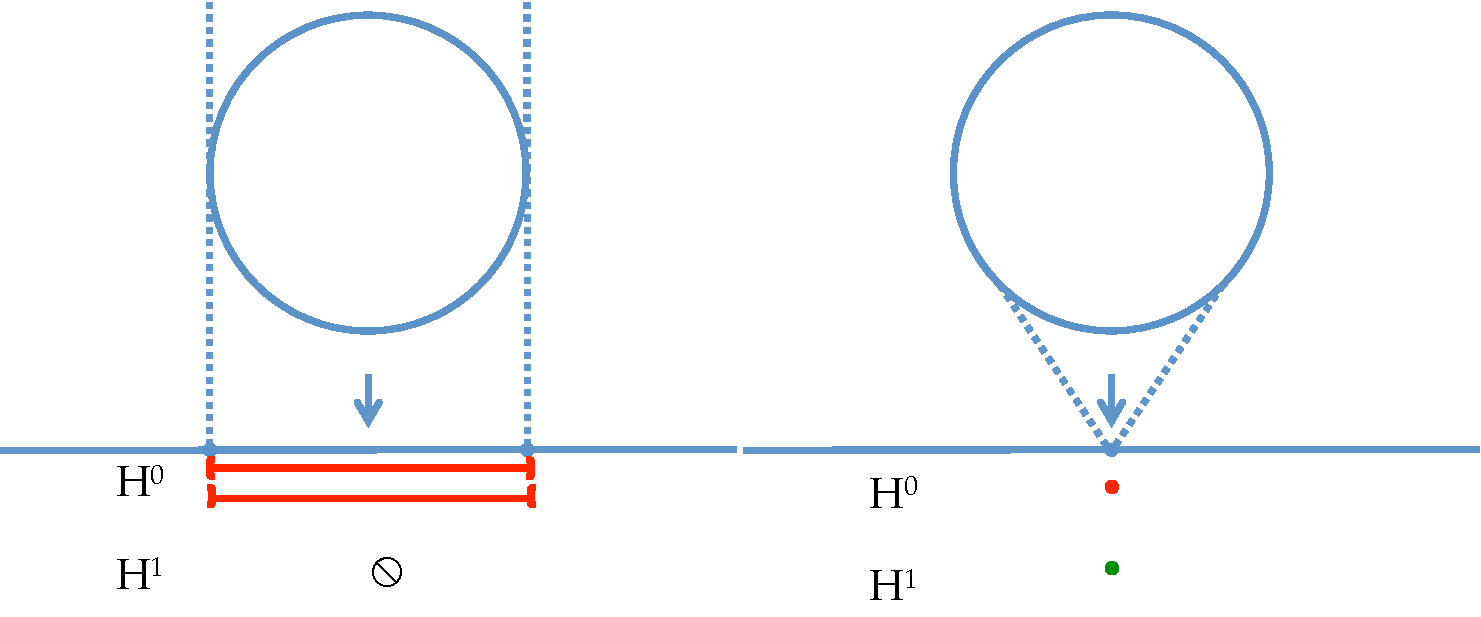
\includegraphics[width=\textwidth]{interleaving_12.pdf}
\caption{Two Maps and their associated Leray Sheaves}
\label{fig:interleaving12}
\end{figure}

Let the map drawn on the left of Figure~\ref{fig:interleaving12} be called $f$ and let the map on the right be called $g$. As already observed in Corollary~\ref{cor:stability}, the presheaves 
\[
H^1F:U\rightsquigarrow H^1(f^{-1}(U);k) \qquad \mathrm{and} \qquad H^1G:U\rightsquigarrow H^1(g^{-1}(U);k)
\]
are $\epsilon$-interleaved for $\epsilon$ larger than the radius of the circle. However, the sheafification of both of these presheaves produce radically different sheaves. 

Recall from Definition~\ref{defn:sheafification} that the sheafification can be viewed as the sheaf of sections of the product over all the stalks mapping down to the base space.
\[
		\xymatrix{ \prod\limits_{x\in \RR} F_x \ar[d]^{\pi} \\ \RR}
\]
For $H^1F$, every stalk is the zero vector space. For $H^1G$, the stalk at $p$ is non-zero and all other ones are zero. Consequently the sheafifications are
\[
		\widetilde{F}^1 \cong 0 \qquad \mathrm{and} \qquad \widetilde{G}^1\cong S_p
\]
where $S_p$ is the skyscraper sheaf at $p$. By lemma~\ref{lem:obstructs}, these two sheaves are not interleaved.

One might conjecture in light of the above example that sheafification is a distance increasing operation. This is not the case. Consider the presheaf $H^1F$ from the example above. One can easily see that it is \emph{not} interleaved with the zero sheaf. However, the sheafification of $H^1F$ is the zero sheaf. So sheafification took two presheaves that were infinite distance apart and returned isomorphic (distance zero) sheaves.

\subsection{Thickening Global Sections}

We will now prove that global sections remain unaffected by this thickening procedure. This provides us with a sheafified version of Lemma~\ref{lem:obstructs}.

\begin{lem}
If $X$ is a metric space such that the closed $\epsilon$-ball is connected for every point of $x$ and the projection map $\epsilon_1:\Bar{\Delta}^{\epsilon}_X\to X$ is a closed map, then thickening preserves global sections, i.e.
\[
	\widetilde{F}^{\epsilon}(X)\cong F(X).
\]
\end{lem}
\begin{proof}
This follows from a simpler version of the Vietoris mapping theorem, stated as Theorem 11.7 of~\cite{Bredon}. Essentially, the Vietoris mapping theorem guarantees that
\[
H^0(X;F)\cong H^0(\Bar{\Delta}^{\epsilon}_X;\epsilon_1^*F)
\]
and since the pushforward $\epsilon_{2*}\epsilon_1^*F$ has the same global sections of $\epsilon_1^*F$ by functoriality (global sections are gotten by pushing forward to a point), then the result follows.
\end{proof}

\subsection{Metric on Sheaves}

\begin{clm}
If $F,G\in\Shv(X)$ are interleaving-distance zero apart, i.e. there is a sequence of $\{\epsilon_n\}$ converging to zero where $F$ and $G$ are $\epsilon_n$ interleaved for each $n$, then $F\cong G$.
\end{clm}
\begin{proof}[Sketch]
We are going to define maps between the \'etal\'e spaces
\[
\varphi:\prod_{x\in X}F_x \to \prod_{x\in X} G_x \qquad \mathrm{and} \qquad \psi:\prod_{x\in X} G_x \to \prod_{x\in X}F_x
\]
with the property that they are inverses of one another.

Given any element $s_x\in F_x$ there exists a $U\ni x$ and a section $s_U$ such that $(s_U)_x=s_x$. However, since $U$ is open, there exists an $r>0$ and $\epsilon_n>0$ such that $B(x,r+2\epsilon_n)\subset U$. This implies in turn that $B(x,r)^{2\epsilon_n}\subset U$. Consequently, there is a lift $s^{2\epsilon_n}_x\in \widetilde{F}^{2\epsilon_n}_x$ of $s_x$, gotten by taking the image of $s_u$ under the following composition:
\[
F(U)\to F(B(x,r+2\epsilon_n))\to F(B(x,r)^{2\epsilon_n})\to \widetilde{F}^{2\epsilon_n}_x
\]

We then define 
\[
\varphi(s_x):=\varphi^{\epsilon_n}_x\circ\widetilde{\eta_{\epsilon_n,2\epsilon_n}}^F_x(s^{2\epsilon_n}_x)
\]
Of course, by the definition of interleaving, we have a natural choice of a lift of $\varphi(s_x)$ to $\widetilde{G}^{\epsilon_n}_x$ given by 
\[
\widetilde{\eta_{\epsilon_n}}^G_x\varphi^{2\epsilon_n}_x(s^{2\epsilon_n}_x),
\]
which by construction has the property that applying $\psi^{\epsilon}_x$ yields $s_x$.

Of course it needs to be checked that such a lift is picked out by the symmetric construction of the map $\psi$. It could have happened that a lift to $\widetilde{G}^{\epsilon_n'}_x$ for $\epsilon_n'\neq \epsilon_n$. However, one only needs to observe that for any sheaf $F$ we have the following commutative diagram for any pair $0<\epsilon_n'<\epsilon_n$:
\[
\xymatrix{\widetilde{F}^{2\epsilon_n} \ar[d] \ar[r] & \widetilde{F}^{\epsilon_n} \ar[d] \ar[r] & F \\
\widetilde{F}^{2\epsilon_n'} \ar[r] & \widetilde{F}^{\epsilon_n'} \ar[ur] & }
\]
Arguing symmetrically and checking continuity of the resulting maps $\varphi$ and $\psi$ completes the proof.
\end{proof}

\begin{thm}[Skeletal Metric Space]
Let $X$ be an arbitrary metric space. The interleaving distance induces an extended metric on the skeleton of the category of sheaves $\Shv(X)$. Here extended means that the value $d(F,G)=\infty$ is allowed, i.e. there is no interleaving between $F$ and $G$ whatsoever.
\end{thm}
\begin{proof}
Recall that the skeleton of a category $\cC$ is a full, isomorphism-dense subcategory $\cS$ in which no two distinct objects are isomorphic. 

If we take $\cC=\Shv(X)$, on which the interleaving distance already defines an extended pseudo-metric, then the above result implies that if $d(F,G)=0$, then $F\cong G$ and hence in a skeletal subcategory $F=G$. This implies that the interleaving distance is an extended metric when restricted to any skeletal subcategory of $\Shv(X)$.
\end{proof}

As one can imagine, the space of sheaves viewed as a metric space can be enormously complicated. Every map $f:X\to\R^n$ has an associated sheaf on $\R^n$, simply by considering the pushforward of the constant sheaf. This includes every possible subspace $Y\subset \R^n$ with the pushforward of the constant sheaf along this inclusion serving as a sort of ``indicator function'' on it. The interleaving distance would give us one notion of distance between all these possible subspaces. In this case, there is a ready comparison to be made with the Gromov-Hausdorff distance between metric spaces, which is more refined than the interleaving distance. However, the interleaving distance also gives a distance between \emph{information} on top of a metric space, where information is encoded via a sheaf. 

\section{The Space of Constructible Sheaves over $\R$}

In this section we will give an explicit description of the space of constructible/cellular sheaves on $\R$ with the interleaving distance as a metric. It turns out that one can use the indecomposable sheaves to give a set of ``coordinates'' on this space. It will turn out that the space resembles a disjoint union of configuration spaces, where there the components are divvied up by global sections, i.e. $H^0$. A comparison to McDuff's construction of the tangent space use a configuration space of points, where points can disappear, is made.

First we recall the definition of constructible sheaf pertinent to this section. Because there are competing, more general notions of a constructible sheaf, we will use slightly different terminology.

\begin{defn}\index{category!of definable sheaves}\index{sheaf!definable}
Let $\Shv_d(\R)$ denote the \textbf{category of definable sheaves} over the real line $\R$, equipped with the usual Euclidean topology. Specifically, a sheaf $F$ will be regarded as a contravariant functor from the open set category with the necessary gluing properties. Such a sheaf $F$ is \textbf{definable} if $\R$ can be written as the finite union of open intervals and points 
\[
\R=(-\infty,a_0)\cup \{a_0\}\cup \cdots (a_i,a_{i+1}) \cdots \cup \{a_n\} \cup (a_n,\infty)
\]
such that when restricted to each interval the sheaf is locally constant. We do \textbf{not} assume that every sheaf is constructible with respect to the same set of intervals.

We will find it convenient to work with a subcategory of this category given by the definable sheaves with \textbf{finite support}, $\Shv_{d,f}(X)$, where the sheaf must restrict to zero on the two half-open intervals including $\pm\infty$.
\end{defn}

As already established in this thesis, such a sheaf is completely described via a zig-zag of vector spaces and linear maps
\[
F(a_0)\leftarrow F(x_0) \rightarrow F(a_1) \leftarrow F(x_1)\rightarrow \cdots \leftarrow F(x_n) \rightarrow F(a_n)
\]
where we have abbreviated the intervals and points by using $a$'s and $x$'s along with subscripts appropriately.

By Gabriel's theorem, we know that such a diagram amounts to a representation of an $A_n$-type quiver and can be decomposed into finitely many indecomposable representations. These indecomposables, in view of the cell structure, can be regarded as one of the following sheaves:
\begin{itemize}
\item $k_{[x_i,x_j]}$ --- the constant sheaf on the closed interval $[x_i,x_j]$
\item $k_{(x_i,x_j)}$ --- the constant sheaf on the open interval $(x_i,x_j)$
\item $k_{[x_i,x_j)}$ --- the constant sheaf on the half-open interval $[x_i,x_j)$
\item $k_{(x_i,x_j]}$ --- the constant sheaf on the half-open interval $(x_i,x_j]$
\item $k_{\R}$ --- the constant sheaf supported on the whole real line $\R$
\item $S_x$ --- the skyscraper sheaf concentrated on the vertex $x$
\end{itemize}
The skyscraper sheaf, $S_x$, is just a special instance of the constant sheaf on a closed interval $[x_i,x_j]$ where $x_i=x_j$. As such, we will not always distinguish the skyscraper sheaf from the constant sheaf on the closed interval. Similarly, one can view the constant sheaf on $\R$, $k_{\R}$, as a degenerate version of the open interval. 

To keep the notation clean and free ourselves from a particular declaration of cell structure on the real line, we will speak of the \textbf{four indecomposable sheaves} on the real line:
\[
k_{[b,d]} \qquad k_{(b,d)} \qquad k_{[b,d)} \qquad k_{(b,d]}
\]

\begin{rmk}
The constant sheaf, $k_{\R}$, and any of the others where $b$ or $d$ is $\pm\infty$ are excluded from the category of definable sheaves with finite support.
\end{rmk}

In the following sections it will be paramount to understand when there is and isn't a non-zero map of sheaves between these four types.

\begin{prop}[D\'evissage for 1D Indecomposable Sheaves]\label{prop:devissage}
We have the following explicit characterizations for the space of sheaf morphisms:
\begin{itemize}
\item For closed intervals $I_1=[b_1,d_1]$ and $I_2=[b_2,d_2]$ we have
\begin{equation*}
 \Hom_{\Shv}(k_{I_1},k_{I_2})=
\begin{cases}
 k & \text{if } I_2\subseteq I_1, \\
0 & \text{o.w.}
\end{cases}
\end{equation*}
\item For open intervals $I_1=(b_1,d_1)$ and $I_2=(b_2,d_2)$ we have
\begin{equation*}
 \Hom_{\Shv}(k_{I_1},k_{I_2})=
\begin{cases}
 k & \text{if } I_1\subseteq I_2, \\
0 & \text{o.w.}
\end{cases}
\end{equation*}
\item For half open intervals of the form $I_n=[b_n,d_n)$ we have
\begin{equation*}
 \Hom_{\Shv}(k_{I_1},k_{I_2})=
\begin{cases}
 k & \text{if } b_1\leq b_2 \text{ and } b_2<d_1\leq d_2 , \\
0 & \text{o.w.}
\end{cases}
\end{equation*}
\item For half open intervals of the form $I_n=(b_n,d_n]$ we have
\begin{equation*}
 \Hom_{\Shv}(k_{I_1},k_{I_2})=
\begin{cases}
 k & \text{if } b_2\leq b_1 \text{ and } b_1<d_2\leq d_1, \\
0 & \text{o.w.}
\end{cases}
\end{equation*}
\item For a closed interval $I_1=[b_1,d_1]$ and any non-compact interval $I_2$
\begin{equation*}
 \Hom_{\Shv}(k_{I_1},k_{I_2})= 0
\end{equation*}
\end{itemize}
\end{prop}
\begin{proof}
The calculations all follow from considering the behavior of a cellular sheaf map near the endpoints of the above indecomposables. Specifically, in a small enough neighborhood of any point in the real line, an indecomposable cellular sheaf has one of the following three forms, possibly after reflection.
\[
M=\quad 0\leftarrow k \rightarrow k
\]
\[
U=\quad k\leftarrow k \rightarrow k
\]
\[
H=\quad k\leftarrow 0 \rightarrow 0
\]
Clearly there are non-zero natural transformations $H\Rightarrow U\Rightarrow M$, but every natural transformation $M\Rightarrow U\Rightarrow H$ must be zero.
\end{proof}

\begin{rmk}[D\'evissage for Constructible Sheaves]
In David Nadler's beautiful application of constructible sheaves to the study of the Fukaya category~\cite{nadler-catmorse}, he refers to the diagram
$$
\xymatrix{
\Shv(V) \ar@/^2pc/[rr]^-{j_!}\ar@/_2pc/[rr]^-{j_*} && \ar[ll]_-{j^! \simeq j^*} \Shv(X)  \ar@/^2pc/[rr]^-{i^*} 
\ar@/_2pc/[rr]^-{i^!} 
&& \ar[ll]_-{i_! \simeq i_*} \Shv(Y)
}
$$
as the ``d\'evissage pattern for constructible sheaves'' --- an ode to Grothendieck's method for studying \emph{coherent} sheaves. Here $j:V\to X$ is the inclusion of an open set and $i:Y:=X-V\to X$ is the inclusion of the closed complement. Here the categories $\Shv(-)$ refer to the full differential graded category of constructible complexes of sheaves, $H^0$ of which is the usual derived category.
\end{rmk}


\subsection{Interleavings and Dynamics on Indecomposable Sheaves}
\index{interleaving!of sheaves!over the real line}
Since indecomposable sheaves are the underlying elements that build up a sheaf, we investigate the behavior of each of these sheaves under epsilon-thickening. We summarize the result of each of these calculations below:
\begin{itemize}
\item If $F=k_{[b,d]}$ and $\epsilon \geq 0$, then $\widetilde{F}^{\epsilon}=k_{[b-\epsilon,d+\epsilon]}$.
\item If $F=k_{(b,d)}$ and $0\leq \epsilon < d-b$, then $\widetilde{F}^{\epsilon}=k_{(b+\epsilon,d-\epsilon)}$. If $d-b\leq \epsilon$, then $\widetilde{F}^{\epsilon}=0$.
\item If $F=k_{[b,d)}$ and $\epsilon \geq 0$, then $\widetilde{F}^{\epsilon}=k_{[b-\epsilon,d-\epsilon]}$.
\item If $F=k_{(b,d]}$ and $\epsilon \geq 0$, then $\widetilde{F}^{\epsilon}=k_{[b+\epsilon,d+\epsilon]}$.
\end{itemize}
With these calculations in hand, we can then discuss distance between these sheaves.
\begin{itemize}
\item The sheaf $k_{[b,d]}$ is interleaving distance $r=(d-b)/2$ from the skyscraper sheaf $S_{m}$ where $m=(d+b)/2$ --- the midpoint --- and infinite distance from any of the other three types of indecomposables, as well as the zero sheaf.
\item The sheaf $k_{(b,d)}$ is interleaving distance $r=(d-b)/2$ from the zero sheaf $0$.
\item The sheaves $k_{[b,d)}$ and $k_{(b.d]}$ are interleaving distance $r=(d-b)/2$ from the zero sheaf $0$.
\end{itemize}

We now give the supporting arguments for these calculations.

\begin{prop}
If $F=k_{[b,d]}$ and $\epsilon\geq 0$, then $\widetilde{F}^{\epsilon}=k_{[b-\epsilon,d+\epsilon]}$.
\end{prop}
\begin{proof}
To construct $\widetilde{F}^{\epsilon}$ it suffices to consider the stalks of the thickened pre-sheaf. It suffices to consider the extreme points. Consider the point $x=b-\epsilon$, then any ball $B(x,r)$ has the property that $[b,d]\cap B(x,r)^{\epsilon}=[b,b+r)\neq\emptyset$. Since $F$ is defined as the pushforward of the constant sheaf along $j:X=[b,d]\hookrightarrow \R$, then $F^{\epsilon}(B(x,r))=k_X([b,b+r))=k$. This proves that $F_x\cong k$.
\end{proof}

\begin{prop}
If $F=k_{(b,d)}$ and $0\leq \epsilon < d-b$, then $\widetilde{F}^{\epsilon}=k_{(b+\epsilon,d-\epsilon)}$. If $d-b\leq \epsilon$, then $\widetilde{F}^{\epsilon}=0$.
\end{prop}
\begin{proof}
If $j:W=(b,d)\hookrightarrow \R$ denotes the inclusion of the open interval, then we can identify $F=j_! k_W$. Here $j_!$ denotes the pushforward with compact supports functor. For the inclusion of a locally closed subspace $W$ into a general topological space $X$ \cite{iversen} provides a precise description. For a sheaf $F$ on $W$ the sheaf $j_!F$ has sections on an open set $U$ given by
\[
\Gamma(U,j_!F):=\{s\in \Gamma(W\cap U,F) \,|\, \supp(s) \, \mathrm{closed}\,\mathrm{rel.}\, U\}
\]
The support of a section is the set of points where a section has non-vanishing stalks.

For an open set $U\subset\R$, we can describe the sheaf pertinent to us even more explicitly: $j_! k_W(U)$ is non-zero if and only if there is a closed set $Y$ such that $U\subset Y\subset W$ --- we say that $U$ is \textbf{completely contained} in $W$. Note that $W=(b,d)$ is \emph{not} completely contained in itself, so in particular $(b,d)$ is assigned the zero vector space by $j_!k_W$.

Consequently, any point $x$ within distance $\epsilon$ of the boundary of $(b,d)$ will fail to possess a ball $B(x,r)$ such that $B(x,r)^{\epsilon}$ is completely contained in $(b,d)$. Thus we say that $(b,d)$ is ``eroded'' by distance $\epsilon$.
\end{proof}

\begin{prop}
If $F=k_{[b,d)}$ and $\epsilon \geq 0$, then $\widetilde{F}^{\epsilon}=k_{[b-\epsilon,d-\epsilon]}$.
\end{prop}
\begin{proof}
This follows by considering each of the above arguments separately about each endpoint.
\end{proof}

Because the other case is obviously symmetric, we omit a separate argument.

An extremely important observation that distinguishes interleavings of sheaves from the usual context of an interleavings of persistence modules~\cite{bauer2013induced} is that the sheaf $k_{[b,d]}$ is not interleaved with the zero sheaf. This follows from the fact that the space of global sections is preserved by thickening.

\subsection{Coordinates for the Category of Sheaves}
\index{category!of sheaves!coordinates}

We can now use the decomposition theorem for constructible sheaves over the real line to give explicit coordinates for each isomorphism class of a definable sheaf with finite support.

Let $\HH=\{(x,y)\in \R^2 \,|\, y\geq 0 \}$ denote the closed upper half plane. To each of the four indecomposable sheaves with finite support --- $k_{[b,d]}$, $k_{(b,d)}$, $k_{[b,d)}$, and $k_{(b,d]}$ --- we can associate a point in $\HH$ as follows:
\[
I \rightsquigarrow (x,y)=(m(I),r(I)):=(\frac{b+d}{2},\frac{d-b}{2})
\]
Here $I$ is a stand-in for any of the four types of indecomposable sheaves. The variable names $m$ and $r$ are meant to connote the midpoint and the radius, respectively, of the underlying bar in the ``barcode''. One can then associate to any definable sheaf $F$ with finite support the following coordinates
\[
F\cong \bigoplus_{k=1}^n k_{I_k}\rightsquigarrow \{(m(I_1),r(I_1)),\cdots,(m(I_n),r(I_n))\}\in \HH^{n_1} \sqcup \HH^{n_2} \sqcup \HH^{n_3} \sqcup \HH^{n_4}
\]
where $n_1,n_2,n_3,n_4$ refers to the number of closed, open, half-open on the right and half-open on the left indecomposables occurring in the decomposition for $F$, respectively. Of course, $n=n_1+n+2+n_3+n_4$. 

As presented, the space has too many points for the simple reason that the line $r=0$ in $\HH$ must be identified with the zero sheaf for the non-closed indecomposable types. To capture the full category of sheaves we must append a distinguished basepoint $\star$ to represent the zero sheaf, quotient the upper half plane so as to identify $\{r=0\}\sim \{\star\}$ and then form a few infinite symmetric products. The first part is simple. We define
\[
Z:=(\HH\sqcup \{\star\})/\sim \qquad \mathrm{where} \qquad (m,r)\sim \star \,\,\mathrm{iff}\,\, r=0.
\]
The next construction begins by observing that $Z$ is naturally a pointed space, where $\star$ serves as the distinguished basepoint. To every pointed space we can associate a new space called the infinite symmetric product.

\begin{defn}
 Recall that the \textbf{$n$-fold symmetric product} of $X$, denoted $SP_n(X)$, is given by forming the $n$-fold Cartesian product and quotienting out by the action of the symmetric group, i.e. $SP_n(X):=X^n/\Sigma_n$. 

 Let $Z$ be a pointed topological space, whose distinguished point is $\star$. There is a system of embeddings $Z^n\hookrightarrow Z^{n+1}$ giuven by sending any point 
\[
(z_1,\ldots,z_n) \mapsto (z_1,\ldots,z_{n+1},\star).
\] 
This embedding descends to an embedding $SP_n(Z)\hookrightarrow SP_{n+1}(Z)$, which forms a directed system of spaces. The \textbf{infinite symmetric product} $SP(Z)$ is the direct limit of this system, i.e.
\[
SP(Z)=\varinjlim_{n>0}SP_n(Z).
\]
\end{defn}

We can now state a theorem.

\begin{thm}
Isomorphism classes of $\Shv_{d,f}(\R)$ are in bijective correspondence with points in the following space:
\[
\BB:=\bigsqcup_{n>0}SP_n(\HH)\times \left(SP(Z)\bigvee_{\star} SP(Z) \bigvee_{\star} SP(Z)\right)
\]
\end{thm}

\begin{rmk}
If one could show that the topology induced by the interleaving distance made $\HH$ and $Z$ into cell complexes, then the Dold-Thom theorem would tell us the singular homology of the space of definable sheaves on the real line is isomorphic to a countably infinite number of copies of $\ZZ$ in degree zero and zero in all higher degrees.
\end{rmk}

It remains to be seen what geometry is induced on $\BB$ by pulling back the interleaving distance. Conjecturally, this should be accomplished by the bottleneck distance~\cite{chazal2009proximity,bauer2013induced}, with the stipulation that only points in $SP(Z)$ can be matched with zero.

\subsection{Towards a Bottleneck Distance for Sheaves}

We now investigate simpler descriptions of the interleaving distance for definable sheaves with finite support on the real line. Our goal is to establish a connection between the interleaving distance for sheaves and the bottleneck distance, which we now define.

\begin{defn}[The Bottleneck Distance]\index{bottleneck distance}
Let $\Delta_+:=\{(x,y)\in\R^2| x\leq y\}$ be equipped with the sup norm 
\[
d_{\infty}(p,p')=\sup\{|x_1-x_2|,|y_1-y_2|\}
\]
A multiset $D$ in $\Delta_+$ is a subset $|D|$ of $\Delta_+$ equipped with a multiplicity function $\mu:|D|\to \NN$. Any multiset can be considered as a set via disjoint unions
\[
D=\bigcup_{p\in |D|}\coprod_{i=1}^{\mu(p)}\{p\}.
\]
A multi-bijection $m:D\to D'$ is a bijection between the underlying sets, where if $\mu(p)=k$, then the underlying set has $k$ elements corresponding to $p$. The \textbf{bottleneck distance} is a distance between multisets defined by the formula
\[
d_B(D,D'):=\inf_{m}\sup_{p\in D} d_{\infty}(p,p').
\]
\end{defn}

In usual sub-level set persistence, the multisets $D$ consist of the diagonal $\Delta=\{(x,x)\}$, equipped with infinite multiplicity, and the points $(b,d)$ corresponding to the interval modules $k_{[b,d)}$ making up the interval decomposition of theorem \ref{thm:crawleyboevey}. The stipulation that the diagonal has infinite multiplicity reflects the fact that for half-open intervals, the module can be interleaved with zero. For sheaves, the obstruction by global sections result implies that the number of points corresponding to indecomposables $k_{[b,d]}$ is an invariant of the multi-set --- infinite multiplicity of the diagonal cannot be used there. Nevertheless, we can describe the geometry there in our choice of coordinates.

\begin{lem}
Suppose $F=k_{[m_1-r_1,m_1+r_1]}$ and $G=k_{[m_2-r_2,m_2+r_2]}$ are two indecomposable sheaves supported over closed intervals, then the interleaving distance for $F$ and $G$ is their distance in a taxicab metric on $\HH$, i.e.
\[
d(k_{[m_1-r_1,m_1+r_1]},k_{[m_2-r_2,m_2+r_2]})=|m_1-m_2|+|r_1-r_2|.
\]
\end{lem}
\begin{rmk}
If we write $[m_1-r_1,m_1+r_1]=:[b_1,d_1]$ and $[m_2-r_2,m_2+r_2]=:[b_2,d_2]$ then the taxicab metric specializes to a sup-norm on the space $\{(b,d)\in\R^2\,|\,b\leq d\}$, that is to say
\[
|m_1-m_2|+|r_1-r_2|=\sup\{|b_1-b_2|,|d_1-d_2|\},
\]
which is a special instance of the bottleneck distance on persistence diagrams.
\end{rmk}
\begin{proof}
Without loss of generality we can assume that $m_1\leq m_2$. We know that there can only be a non-zero map from $F^{\epsilon}\to G$ if $[m_2-r_2,m_2+r_2]\subset [m_1-r_1-\epsilon,m_1+r_1+\epsilon]$, i.e. if $\epsilon\geq (m_2-m_1)+(r_2-r_1)$. Similarly, there is a non-zero map $G^{\epsilon}\to F$ only if $\epsilon\geq (m_2-m_1)+(r_1-r_2)$. Since in order for a non-zero interleaving to exist both maps must be non-zero, we conclude that
\[
\epsilon=\sup\{(m_2-m_1)+(r_2-r_1),(m_2-m_1)+(r_1-r_2)\}=m_2-m_1 + |r_1-r_2|.
\]
This proves that there is a non-zero interleaving for this value of $\epsilon$. However, the interleaving distance is the infimum over all such $\epsilon$. However, for any smaller $\epsilon$ one of the maps $\varphi_{\epsilon}$ or $\psi_{\epsilon}$ must be zero. However, global sections obstructs such a pair of maps from defining an interleaving, since for every $\epsilon$ the maps
\[
\eta^F_{2\epsilon}:F^{2\epsilon}(X) \to F(X) \qquad \mathrm{and} \qquad \eta^G_{2\epsilon}:G^{2\epsilon}(X) \to G(X)
\]
are non-zero. They are, in fact, the identity map $\id:k\to k$.
\end{proof}

The situation for constant sheaves supported on half-open intervals or the open interval is more complicated since they have no global sections and can be interleaved with the zero sheaf.

\begin{lem}\label{lem:distance_from_0}
Suppose $F$ and $G$ are each interleaved with the zero sheaf, i.e. $d(F,0),d(G,0)<\infty$. Then the interleaving distance between $F$ and $G$ is bounded above by the greater of the two distances from zero,
\[
d(F,G)\leq \sup\{d(F,0),d(G,0)\}.
\]
\end{lem}
\begin{proof}
Choose any $\epsilon\geq \sup\{d(F,0),d(G,0)\}$, then the zero maps define an $\epsilon$ interleaving, factoring through zero, between $F$ ang $G$. Since the interleaving distance is the infimum, the inequality follows.
\end{proof}

We can use the above lemma to establish what the interleaving distance between pairs of sheaves of the other three types looks like.

\begin{lem}
Let $F=k_{[m_1-r_1,m_1+r_1)}$ and $G=k_{[m_2-r_2,m_2+r_2)}$ be indecomposable sheaves supported on half-open intervals, then
\[
 d(k_{[m_1-r_1,m_1+r_1)},k_{[m_2-r_2,m_2+r_2)})=\inf\{\max(r_1,r_2),|m_1-m_2|+|r_1-r_2|\}
\]
\end{lem}
\begin{proof}
Without loss of generality, we assume that $F=k_{[-R,R)}$ and $G=k_{[m-r,m+r)}$ where $m\geq 0$. This can be done since the $\epsilon$-thickening operation simply translates sheaves of this form to the left by $\epsilon$. In view of lemma \ref{lem:distance_from_0} it suffices to consider the possible values for $m$ and $r$ such that $G^{\epsilon}$ admits a non-zero map to $F$. By proposition \ref{prop:devissage} we can determine precisely what inequalities $\epsilon$ must satisfy.

First we assume that $r\leq R$. In this case, the inequalities are
\[
-r-R\leq m-\epsilon \leq r-R \qquad \mathrm{and} \qquad R-r \leq m+\epsilon < R+r.
\]
The first set of inequalities bounds when $G^{\epsilon}\to F$ can be non-zero and the second set of inequalities bounds when $F^{\epsilon}\to G$ can be non-zero. The smallest such $\epsilon$ that satisfies the first set is $\epsilon=m+R-r$, which only satisfies the second set if $m< R$. For these values of $m$ and $r$, there is the smallest non-zero interleaving, so the distance is
\[
d(F,G)=m+R-r.
\]
Similarly for $r\geq R$, $\epsilon=m+r-R$ is the smallest possible value for $G^{\epsilon}\to F$ to be non-zero. Requiring $F^{\epsilon}\to G$ to be non-zero as well implies that $m\leq R$ and for these values of $m$ and $r$ the distance is
\[
d(F,G)=m+r-R.
\]
Consequently, wherever a non-zero interleaving is possible, the smallest such value is given in the desired taxicab form $m+|r-R|$. Now we can apply lemma \ref{lem:distance_from_0} to determine whether the non-zero interleavings are the smallest possible. We split into two cases. Suppose $r\leq R$, then $m+R-r\leq R$ ---  the largest distance from zero --- when $m\leq r$, precisely where we determined a non-zero interleaving exists. Similarly if $R\leq r$, then we have that $m+r-R\leq r$ precisely if $m\leq R$.
\end{proof}

With this evidence in hand, we believe a version of the isometry theorem~\cite{lesnick-thesis,bubenik2012categorification,bauer2013induced} should hold for definable sheaves with finite support over the real line. However, we must delay this for another time.
